\documentclass[11pt,twoside]{article}
\usepackage{graphicx}

\pagestyle{myheadings}

% -----------------------------------------------------------------------------
% ? Document identification
\newcommand{\stardoccategory}  {Starlink User Note}
\newcommand{\stardocinitials}  {SUN}
\newcommand{\stardocsource}    {sun213.4}
\newcommand{\stardocnumber}    {213.4}
\newcommand{\stardocauthors}   {G. Privett, T. Jenness, H. Matthews, V. Barnard}
\newcommand{\stardocdate}      {10 August 2012}
\newcommand{\stardoctitle}     {FLUXES\\[1ex]
                                JCMT Position and Flux Density Calibration}
\newcommand{\stardocversion}   {Version 1.1}
\newcommand{\stardocmanual}    {User's Manual}
\newcommand{\stardocabstract}  {
FLUXES calculates approximate {\bf topocentric positions} of the planets and also
{\bf integrated flux densities} of five of them at several wavelengths.
These provide calibration information at the effective frequencies and
beam-sizes employed by the UKT14 and SCUBA receivers on the
JCMT telescope based on Mauna Kea, Hawaii.

The FLUXNOW command, runs FLUXES for the current time and date.
This allows you to obtain planetary positions and flux levels quickly.
}
% ? End of document identification

% -----------------------------------------------------------------------------

\newenvironment{myquote}{\begin{quote}\begin{small}}{\end{small}\end{quote}}


% +
%  Name:
%     sun.tex
%
%  Purpose:
%     Template for Starlink User Note (SUN) documents.
%     Refer to SUN/199
%
%  Authors:
%     AJC: A.J.Chipperfield (Starlink, RAL)
%     BLY: M.J.Bly (Starlink, RAL)
%     PWD: Peter W. Draper (Starlink, Durham University)
%
%  History:
%     17-JAN-1996 (AJC):
%        Original with hypertext macros, based on MDL plain originals.
%     16-JUN-1997 (BLY):
%        Adapted for LaTeX2e.
%        Added picture commands.
%     13-AUG-1998 (PWD):
%        Converted for use with LaTeX2HTML version 98.2 and
%        Star2HTML version 1.3.
%     {Add further history here}
%
% -

\newcommand{\stardocname}{\stardocinitials /\stardocnumber}
\markboth{\stardocname}{\stardocname}
\setlength{\textwidth}{160mm}
\setlength{\textheight}{230mm}
\setlength{\topmargin}{-2mm}
\setlength{\oddsidemargin}{0mm}
\setlength{\evensidemargin}{0mm}
\setlength{\parindent}{0mm}
\setlength{\parskip}{\medskipamount}
\setlength{\unitlength}{1mm}

% -----------------------------------------------------------------------------
%  Hypertext definitions.
%  ======================
%  These are used by the LaTeX2HTML translator in conjunction with star2html.

%  Comment.sty: version 2.0, 19 June 1992
%  Selectively in/exclude pieces of text.
%
%  Author
%    Victor Eijkhout                                      <eijkhout@cs.utk.edu>
%    Department of Computer Science
%    University Tennessee at Knoxville
%    104 Ayres Hall
%    Knoxville, TN 37996
%    USA

%  Do not remove the %begin{latexonly} and %end{latexonly} lines (used by
%  LaTeX2HTML to signify text it shouldn't process).
%begin{latexonly}
\makeatletter
\def\makeinnocent#1{\catcode`#1=12 }
\def\csarg#1#2{\expandafter#1\csname#2\endcsname}

\def\ThrowAwayComment#1{\begingroup
    \def\CurrentComment{#1}%
    \let\do\makeinnocent \dospecials
    \makeinnocent\^^L% and whatever other special cases
    \endlinechar`\^^M \catcode`\^^M=12 \xComment}
{\catcode`\^^M=12 \endlinechar=-1 %
 \gdef\xComment#1^^M{\def\test{#1}
      \csarg\ifx{PlainEnd\CurrentComment Test}\test
          \let\html@next\endgroup
      \else \csarg\ifx{LaLaEnd\CurrentComment Test}\test
            \edef\html@next{\endgroup\noexpand\end{\CurrentComment}}
      \else \let\html@next\xComment
      \fi \fi \html@next}
}
\makeatother

\def\includecomment
 #1{\expandafter\def\csname#1\endcsname{}%
    \expandafter\def\csname end#1\endcsname{}}
\def\excludecomment
 #1{\expandafter\def\csname#1\endcsname{\ThrowAwayComment{#1}}%
    {\escapechar=-1\relax
     \csarg\xdef{PlainEnd#1Test}{\string\\end#1}%
     \csarg\xdef{LaLaEnd#1Test}{\string\\end\string\{#1\string\}}%
    }}

%  Define environments that ignore their contents.
\excludecomment{comment}
\excludecomment{rawhtml}
\excludecomment{htmlonly}

%  Hypertext commands etc. This is a condensed version of the html.sty
%  file supplied with LaTeX2HTML by: Nikos Drakos <nikos@cbl.leeds.ac.uk> &
%  Jelle van Zeijl <jvzeijl@isou17.estec.esa.nl>. The LaTeX2HTML documentation
%  should be consulted about all commands (and the environments defined above)
%  except \xref and \xlabel which are Starlink specific.

\newcommand{\htmladdnormallinkfoot}[2]{#1\footnote{#2}}
\newcommand{\htmladdnormallink}[2]{#1}
\newcommand{\htmladdimg}[1]{}
\newcommand{\hyperref}[4]{#2\ref{#4}#3}
\newcommand{\htmlref}[2]{#1}
\newcommand{\htmlimage}[1]{}
\newcommand{\htmladdtonavigation}[1]{}

\newenvironment{latexonly}{}{}
\newcommand{\latex}[1]{#1}
\newcommand{\html}[1]{}
\newcommand{\latexhtml}[2]{#1}
\newcommand{\HTMLcode}[2][]{}

%  Starlink cross-references and labels.
\newcommand{\xref}[3]{#1}
\newcommand{\xlabel}[1]{}

%  LaTeX2HTML symbol.
\newcommand{\latextohtml}{\LaTeX2\texttt{HTML}}

%  Define command to re-centre underscore for Latex and leave as normal
%  for HTML (severe problems with \_ in tabbing environments and \_\_
%  generally otherwise).
\renewcommand{\_}{\texttt{\symbol{95}}}

% -----------------------------------------------------------------------------
%  Debugging.
%  =========
%  Remove % on the following to debug links in the HTML version using Latex.

% \newcommand{\hotlink}[2]{\fbox{\begin{tabular}[t]{@{}c@{}}#1\\\hline{\footnotesize #2}\end{tabular}}}
% \renewcommand{\htmladdnormallinkfoot}[2]{\hotlink{#1}{#2}}
% \renewcommand{\htmladdnormallink}[2]{\hotlink{#1}{#2}}
% \renewcommand{\hyperref}[4]{\hotlink{#1}{\S\ref{#4}}}
% \renewcommand{\htmlref}[2]{\hotlink{#1}{\S\ref{#2}}}
% \renewcommand{\xref}[3]{\hotlink{#1}{#2 -- #3}}
%end{latexonly}
% -----------------------------------------------------------------------------
% ? Document specific \newcommand or \newenvironment commands.
% ? End of document specific commands
% -----------------------------------------------------------------------------
%  Title Page.
%  ===========
\renewcommand{\thepage}{\roman{page}}
\begin{document}
\thispagestyle{empty}

%  Latex document header.
%  ======================
\begin{latexonly}
   CCLRC / \textsc{Rutherford Appleton Laboratory} \hfill \textbf{\stardocname}\\
   {\large Particle Physics \& Astronomy Research Council}\\
   {\large Starlink Project\\}
   {\large \stardoccategory\ \stardocnumber}
   \begin{flushright}
   \stardocauthors\\
   \stardocdate
   \end{flushright}
   \vspace{-4mm}
   \rule{\textwidth}{0.5mm}
   \vspace{5mm}
   \begin{center}
   {\Huge\textbf{\stardoctitle \\ [2.5ex]}}
   {\LARGE\textbf{\stardocversion \\ [4ex]}}
   {\Huge\textbf{\stardocmanual}}
   \end{center}
   \vspace{5mm}

% ? Add picture here if required for the LaTeX version.
%   e.g. \includegraphics[scale=0.3]{filename.ps}
% ? End of picture

% ? Heading for abstract if used.
   \vspace{10mm}
   \begin{center}
      {\Large\textbf{Abstract}}
   \end{center}
% ? End of heading for abstract.
\end{latexonly}

%  HTML documentation header.
%  ==========================
\begin{htmlonly}
   \xlabel{}
   \begin{rawhtml} <H1 ALIGN=CENTER> \end{rawhtml}
      \stardoctitle\\
      \stardocversion\\
      \stardocmanual
   \begin{rawhtml} </H1> <HR> \end{rawhtml}

% ? Add picture here if required for the hypertext version.
%   e.g. \includegraphics[scale=0.7]{filename.ps}
% ? End of picture

   \begin{rawhtml} <P> <I> \end{rawhtml}
   \stardoccategory\ \stardocnumber \\
   \stardocauthors \\
   \stardocdate
   \begin{rawhtml} </I> </P> <H3> \end{rawhtml}
      \htmladdnormallink{CCLRC}{http://www.cclrc.ac.uk} /
      \htmladdnormallink{Rutherford Appleton Laboratory}
                        {http://www.cclrc.ac.uk/ral} \\
      \htmladdnormallink{Particle Physics \& Astronomy Research Council}
                        {http://www.pparc.ac.uk} \\
   \begin{rawhtml} </H3> <H2> \end{rawhtml}
      \htmladdnormallink{Starlink Project}{http://www.starlink.ac.uk/}
   \begin{rawhtml} </H2> \end{rawhtml}
   \htmladdnormallink{\htmladdimg{source.gif} Retrieve hardcopy}
      {http://www.starlink.ac.uk/cgi-bin/hcserver?\stardocsource}\\

%  HTML document table of contents.
%  ================================
%  Add table of contents header and a navigation button to return to this
%  point in the document (this should always go before the abstract \section).
  \label{stardoccontents}
  \begin{rawhtml}
    <HR>
    <H2>Contents</H2>
  \end{rawhtml}
  \htmladdtonavigation{\htmlref{\htmladdimg{contents_motif.gif}}
        {stardoccontents}}

% ? New section for abstract if used.
  \section{\xlabel{abstract}Abstract}
% ? End of new section for abstract
\end{htmlonly}

% -----------------------------------------------------------------------------
% ? Document Abstract. (if used)
%  ==================
\stardocabstract
% ? End of document abstract
% -----------------------------------------------------------------------------
% ? Latex document Table of Contents (if used).
%  ===========================================
  \newpage
  \begin{latexonly}
    \setlength{\parskip}{0mm}
    \tableofcontents
    \setlength{\parskip}{\medskipamount}
    \markboth{\stardocname}{\stardocname}
  \end{latexonly}
% ? End of Latex document table of contents
% -----------------------------------------------------------------------------

% ? End of Latex document table of contents
% -----------------------------------------------------------------------------
\cleardoublepage
\renewcommand{\thepage}{\arabic{page}}
\setcounter{page}{1}

\section{Introduction}
\xlabel{INTRODUCTION}
\label{sec:introduction}

FLUXES calculates approximate \textbf{topocentric positions} of the planets and
also \textbf{integrated flux densities} of five of them at a number of
wavelengths for the
\htmladdnormallink{JCMT telescope}{http://www.jach.hawaii.edu/JCMT/home.html}
on Mauna Kea, Hawaii.  These provide calibration information at the effective
frequencies and beam-sizes employed by the UKT14, SCUBA and SCUBA-2
receivers on this telescope.

The filter centre and widths are shown for each wavelength used.  The filter
frequencies are the effective frequencies for 1mm of water vapour.

The calculated planet positions should normally be accurate to better than 1
arcminute. The value for the Moon is less accurate than this, and for critical
applications requiring sub arc-second accuracy you should use a different
method.

The planet positions are estimated using the SLALIB library. See
\xref{SUN/67}{sun67}{} for more details on the SLA\_PLANET library function.

The FLUXNOW command, runs the program for the current time and date.  This gives
you current planetary positions and flux levels for all the planets.

\section{Frequencies, brightness and beam-width}
\xlabel{FREQ}
\label{sec:freq}

The effective frequencies and half-power beam-widths for the filters, and the
brightness temperatures for the planets (except Mars) are read from the plain
text files:

\begin{description}
\item[\mbox{}]\mbox{}
\begin{description}
\item [ukt14\_old.dat] -- for dates before 7-Aug-92.
\item [ukt14.dat] -- for the period 7-Aug-92 to 23-May-96.
\item [scuba.dat] -- for dates after 23-May-96.
\end{description}
\end{description}

The information in the files was supplied by the observatory.
The differences mainly reflect changes in detector/telescope hardware.

The program selects the appropriate {\tt{.dat}} file to use, based on the date
you specify.
The calculated temperature has an rms error of about 0.13K (negligible).

Bear in mind that Saturn can only be used for calibration when the
rings are not open, and the Martian brightness temperatures are probably
only accurate to around $\pm5$\%.

\section{Using FLUXES}
\xlabel{USING}
\label{sec:using}

To run FLUXES or FLUXNOW, type its name (in lower case) after the prompt:

\begin{myquote}
\begin{verbatim}
% fluxes
\end{verbatim}
\end{myquote}

The program first asks you what output you want to generate:

\begin{myquote}
\begin{verbatim}
JCMT FLUXES

POS - Do you require planetary data? (Y/N) /YES/ > Y
FLU - Do you require flux data?      (Y/N) /YES/ > Y
\end{verbatim}
\end{myquote}

In the above example I opted to see both sets of output data.
If you were only interested in the planetary positions, reply ``{\tt{N}}''
to the second prompt.
(Prompts asking for a {\tt{Y/N}} answer can also be answered using
{\tt{true/false}} or {\tt{t/f}} or {\tt{y/n}} --
case is not significant.)

Next, indicate where you want the information displayed or stored:

\begin{myquote}
\begin{verbatim}
SCREEN - Display output to terminal? (Y/N) /YES/ > Y
OFL - Store output in a file?        (Y/N) /NO/ > Y
OUTFILE - Name of output file /'fluxes.dat'/ >

Data will be written to file: /home/user1/gjp/flux/fluxes.dat
\end{verbatim}
\end{myquote}

If you reply ``{\tt{N}}'' to the OFL prompt, the next lines shown won't appear.

Next, you are asked to specify the time and date for which the information
should be derived.
If you set the value of NOW to {\tt{Y}}, the current date
and time are automatically obtained from your computer.
Otherwise, you must specify the time and date yourself, as appears below:

\begin{myquote}
\begin{verbatim}
NOW - Use todays date/time? (Y/N) /YES/ > N

DATE - UT DATE (DD MM YY) /'12 09 96'/ > 16 09 96
TIME - UT TIME (HH MM SS) /'12 00 00'/ > 08 45 00
\end{verbatim}
\end{myquote}

Since you might only require flux and positional information for one planet,
you are given the option of selecting it by specifying a value for the
parameter PLANET.
When prompted, give the name of any planet, the Sun, the Moon,
or `ALL' (meaning all the planets plus the Sun and Moon).
The information requested is then output to the screen and/or to the file
(depending on the values you gave the parameters SCREEN and OFL).
An example of the output generated is:

\begin{myquote}
\begin{verbatim}
Planetary Submillimetre Fluxes for the JCMT

UT:  11:25:55       UT Date:18-Sep-1996     HST: 1:25:55

LST:  0:53:52.8981  Julian:  2450344.976  Epoch: 1996.7145

Body         RA        TRIMRA         Dec       TRIMDEC        GD     AMASS
           (h m s)  (arcsec/sec)    (d m s)  (arcsec/sec)     (au)
SUN     11 44 39.7958  0.0379   + 1 39 35.6411  -0.0161    1.004696  13.375
MERCURY 11 33 12.7569 -0.0334   - 0 15 11.0814   0.0277    0.652113  13.375
VENUS    8 57 54.0821  0.0475   +16 20 20.0995  -0.0096    0.931408  13.375
MARS     8 32  2.5581  0.0268   +19 56 37.7140  -0.0057    2.022076  13.375
JUPITER 18 35 37.5441  0.0021   -23 23 38.9082   0.0001    4.866561  13.375
SATURN   0 21  4.1782 -0.0030   - 0 33 48.7199  -0.0013    8.508145   1.078
URANUS  20 12 44.5684 -0.0008   -20 33 32.2338  -0.0001   19.189787   5.468
NEPTUNE 19 47 41.0764 -0.0004   -20 39 32.1751  -0.0001   29.655347  10.395
PLUTO   16  4 56.5905  0.0008   - 7 52 56.4430  -0.0005   30.327917  13.375
MOON    15 54 32.2690  0.7373   -16 17 35.4393  -0.0368    0.002580  13.375
\end{verbatim}
\end{myquote}

\newpage

\begin{myquote}
\begin{verbatim}
Mars
South pole is Earth-facing; Inclination Angle =  73.30 degrees
Semi-diameter =  2.31 arcsecs    Solid angle =  3.95E-10 sterads
Filter    Centre   Filter   Total   Flux in    Brightness          HPBW
Wavel.     Freq     Width    Flux    beam      Temperature       assumed
micron     (GHz)    (GHz)    (Jy)     (Jy)          (K)          (arcsecs)
 2000     146.0    39.0     52.15     51.81    205.1 +-  0.0       33.8
 1300     221.0    60.0    119.62    117.85    207.1 +-  0.0       22.3
 1100     264.0    60.0    170.56    167.00    208.0 +-  0.0       18.7
  850     350.0    30.0    298.80    287.78    209.3 +-  0.0       14.0
  750     407.0    30.0    402.83    383.11    210.0 +-  0.0       12.1
  600     483.0    51.0    564.65    526.27    210.9 +-  0.0       10.2
  450     677.0    30.0   1093.57    954.64    212.5 +-  0.0        7.3
  350     866.0    30.0   1761.21   1414.15    213.7 +-  0.0        5.7
\end{verbatim}
\end{myquote}

and so on....

If you encounter problems, please ask your system manager to consult
Appendix A.

\section{Planetary brightness and flux density calculations}
\xlabel{PLANET}
\label{sec:planet}

The calibration of the temperature and flux density scales for the
\htmladdnormallink{JCMT}{http://www.jach.hawaii.edu/JCMT/home.html} antenna
ultimately rests on accurate knowledge of the brightness temperatures of the
planets as a function of frequency.
The main planets used are: Mars, Jupiter, Saturn, Uranus, and Neptune.
Brightness and flux values are not provided for Mercury, Venus, or Pluto/Charon.
Mars is used as the primary calibrator; that is, the brightness
temperatures of all other planets are referred to the brightness temperature of
Mars. Since Mars is a solid body, it is relatively secure to use a model of its
brightness temperature as a function of date. This information can then be used
to calibrate observations of the other planets.

Once the brightness temperatures are known, it becomes possible to calculate
the flux density received at the Earth from a given planet, corrected for the
apparent size of the planet and the beam size of the
\htmladdnormallink{JCMT}{http://www.jach.hawaii.edu/JCMT/home.html}
at the frequency being used.
This is done by FLUXES and FLUXNOW.

Historically, FLUXES was developed for use with the bolometer UKT14.
For each of the presently available UKT14 filters the brightness temperature
and total flux density of the planet is calculated, along with the flux density
visible to a 65mm aperture (the standard detector width) -- shown in the
tables under the heading {\tt{Flux in beam}}.
The latter is calculated from the beam width given in the final column -- if
you have reason to believe that the beam width is different, or you have used a
different aperture, you will have to re-do the calculation.

The planetary brightness temperatures used are obtained from the measurements
of Griffin et al. (1986, {\tt{Icarus}}, 65, 244), Orton et al.
(1986, {\tt{Icarus}}, 67, 289),
and Griffin \& Orton (1993, {\tt{Icarus}}, 105, 537). The errors in brightness
temperatures are the rms internal errors of the observations.

From MJD 46040 until MJD 50000 ({\em{i.e.}}\ JD 2450000.5, corresponding to 1995
October 10), FLUXES uses $\lambda350\mu$m Martian brightness temperatures
$T_b$ derived from the model described by Wright (1976, {\tt{Ap.J.}}, 210, 250).
This uses an adjusted model of the thermal
behaviour of Mars' surface and geometric factors to predict the flux received at
the Earth and the whole-disk brightness temperature at 40-day intervals. The
model does not include the effects of dust storms and the Martian polar cap. At
all other times, the model has a maximum uncertainty of within $\pm5$\% . Since
the results for Mars are derived from models, no errors are quoted in the output
of FLUXES.

Before MJD 46040 and, more importantly, since MJD 50000, FLUXES uses a
modification of Wright's rotating cratered asteroid program (Wright,
E.L., 1995; private communication to H.E. Matthews). This reproduces
82\%\ of the $T_b$ values in Table~6 of Wright (1976) exactly (where they are
rounded to the nearest Kelvin), while the other 18\%\ differ by only $\pm1$~K.
A low-precision formula by Van Flandern and Pulkinnen,
(1979, {\tt{Ap.J.Supp.}}, 41, 391)
was used to compute the geometric factors (Mars-Sun
distance $R$, Martian declinations of the Sun and the Earth $D_S$ and $D_E$,
and the difference in Martian right ascensions between the Earth and the Sun
$A_S - A_E$) far into the future.

\begin{figure}
\includegraphics[angle=-90,width=\textwidth]{sun213_fig1.eps}
\vspace*{-0.5cm}
\caption{Martian brightness temperatures}
\label{fig:mars}
\end{figure}

The values of $T_b$ for Mars are calculated for the entire date range
at intervals of 40 days. FLUXES interpolates between the nearest two
values to obtain the value for the requested date and time.
Figure \ref{fig:mars} shows the variation of disk-averaged Martian $\lambda350$-$\mu$m
brightness temperatures over a period of 25.2 years, beginning in late 1975,
calculated using a rotating cratered asteroid model, and corrected for the
microwave background. The differences between this model and the full model
by Wright (1976) over the range for which data is available is shown
dotted below, where the solid horizontal line is 0~K~T$_b$ difference.

Over the interval for which
both the original Wright model and the simplified model are valid, the
differences in brightness temperatures have an rms error of 0.13~K
({\em i.e.}\ negligible) after removing a constant offset of -2.56~K, assumed
due to the microwave background.

\section{Using FLUXNOW}
\xlabel{FLUXNOW}
\label{sec:fluxnow}


FLUXNOW is a script that calls the program FLUXES in such a way that
the results for the current date and time are returned to you without
further input.  For your convenience, the information generated is
placed in a file called {\tt{fluxes.dat}} in your current directory.
If a file of that name already exists, the information is appended to
the existing file.  Note that, as with FLUXES, the FLUXNOW command
which runs the script should be typed at the UNIX prompt in lower case,
as given below:

\begin{myquote}
\begin{verbatim}
% fluxnow
\end{verbatim}
\end{myquote}

\section{Acknowledgements}
\xlabel{ACKNOWLEDGEMENTS}
\label{sec:acknowledgements}

FLUXES was originally developed as part of the
`\htmladdnormallink{JCMT}{http://www.jach.hawaii.edu/JCMT/home.html} Utilities'
package maintained by the \htmladdnormallink{JCMT Software Group}
{http://www.jach.hawaii.edu/jcmt_sw/} at Hilo, Hawaii. It is
loosely based on code originally developed by B.D. Yallop and C.Y. Hohenkerk
of \htmladdnormallink{HM Nautical Almanac Office}{http://www.ast.cam.ac.uk/}.

\clearpage

\appendix
\section{Installation}
\xlabel{INSTALLATION}
\label{sec:installation}

Most of what follows is likely to be of interest to site system managers only
and may be skipped by the rest of us.

The FLUXES/FLUXNOW code and associated files are supplied as a compressed
tar file: {\tt{fluxes.tar.Z}}.  To install FLUXES/FLUXNOW the file must be
uncompressed and the contents extracted to a suitable directory.  On
Starlink systems, this would normally be directory {\tt{/star/fluxes}}. The
operation is:

\begin{myquote}
\begin{verbatim}
% cd /star/fluxes           (or some directory you specify)
% zcat /tmp/fluxes.tar.Z | tar xvf -
\end{verbatim}
\end{myquote}

You must then set an environment variable to identify the type of operating
system you are using. The example given below shows the value of
{\tt{SYSTEM}} needed to create a Solaris version of the software. The values
required for other Starlink supported systems may be found in the files
{\tt{mk}} and {\tt{makefile}}.

\begin{myquote}
\begin{verbatim}
% setenv SYSTEM sun4_Solaris
\end{verbatim}
\end{myquote}

The UNIX `make' facility may then be employed to generate FLUXES in the
current directory, clean up after itself and move the run time system
to the directory from which it will normally be run.  Note that you must
set the environmental variable {\tt{INSTALL}} to reflect the directory
above that in which you want FLUXES and FLUXNOW to be installed. On
most Starlink system this will be directory {\tt{/star}}:

\begin{myquote}
\begin{verbatim}
% setenv INSTALL /star
% ./mk build
% ./mk clean strip
% ./mk install
\end{verbatim}
\end{myquote}

Once this is done you can make FLUXES and FLUXNOW available to you
by inserting:

\begin{myquote}
\begin{verbatim}
if ( -e /star/bin/fluxes/fluxes) then
   alias fluxes /star/bin/fluxes/fluxes.csh
   alias fluxnow /star/bin/fluxes/fluxnow.csh
else
   alias fluxes cat /star/etc/not_installed
   alias fluxnow cat /star/etc/not_installed
endif
\end{verbatim}
\end{myquote}

into your {\tt{/star/etc/cshrc}} file.  The example given assumes that
you have chosen to have the FLUXES executable installed in directory
{\tt{/star/bin/fluxes}}.  Obviously you will need to change this if you
have placed it elsewhere.   On Starlink systems, the
{\tt{/star/etc/cshrc}} file is already set up to run FLUXES.

In addition, the environmental variable {\tt{FLUXES}} in {\tt{fluxes.csh}}
and {\tt{fluxnow.csh}} must be set to name of the directory where the FLUXES
executable resides.  The Starlink installations of FLUXES have this set
automatically during installation.

This behaviour is not the same as that employed for most other Starlink
programs and reflects a compromise between the requirements of the JCMT
observatory and normal Starlink practice.


\section{Running in batch mode}
\xlabel{batch_mode}
\label{sec:batchmode}

Occasionally it would be useful to retrieve planet fluxes without having
to run FLUXES interactively. The current version has been modified so that
in certain circumstances the flux values can be written to ADAM parameters
and retrieved (this is somewhat easier than parsing the output text file).

When FLUXES is run with a single planet name and filter the calculated
flux values for that combination are written to the following
ADAM parameters:

\begin{description}
\item[HPBW:] Half-power beam width used to calculate F\_BEAM (arcsec)
\item[F\_CENTRE:] the centre frequency of the selected filter (GHz)
\item[F\_WIDTH:] the filter width (GHz)
\item[F\_TOTAL:] the total flux (Jy)
\item[F\_BEAM:] the total flux in the beam (Jy)
\item[T\_BRIGHT:] the brightness temperature of the planet (K)
\item[T\_ERROR:] the error in the brightness temperature (K)
\item[SEMI\_DIAM:] Semi-diameter of the selected planet (arcsec).
If `ALL' planets are selected then the parameter will retain the
value of the last planet processed (Neptune)
\item[SOLID\_ANG:] Solid angle of the selected planet (steradians).
If `ALL' planets are selected then the parameter will retain the
value of the last planet processed (Neptune)
\end{description}

If FLUXES is run from the shell (as opposed to running it as a
monolith (see later in the section for information on running fluxes
as a monolith)) the parameter values can be retrieved by using either
the \xref{KAPPA}{sun95}{} \xref{parget}{sun95}{PARGET} command
or, if running from perl, the par\_get routine supplied as part of the
\xref{NDFPERL}{sun222}{} package.

Here is an example, running FLUXES from the command-line with
no output except via the parameter system

\begin{myquote}
\begin{verbatim}
% fluxes pos=no flu=yes screen=no ofl=no now filter=850 apass=no \
       planet=uranus msg_filter=quiet
% parget f_total fluxes
72.4569
\end{verbatim}
\end{myquote}

Note how MSG\_FILTER was used to turn off default messages, and
that the FILTER and PLANET were selected explcitly. Also, useful
output was obtained even though fluxes was instructed to write
to neither the screen or a file (and MSG\_FILTER=QUIET hides
output even if SCREEN=yes).


It is possible to run FLUXES as a monolith but this requires
that the fluxes monolith is run directly (not via the fluxes.csh
shell script), that the envrionment variables
FLUXES and FLUXPWD are set to the location of the fluxes binary
and the current working directory respectively. If it is running
as a monolith (specifically as an I-task) the parameter values can
then be retrieved from the monolith (e.g.\ by using
\xref{STARTCL}{sun186}{adam_message_system_extension} ).

\section{How does FLUXES work?}
\xlabel{howfluxesworks}
\label{sec:howfluxesworks}

In this section we will discuss the actual calculations performed by FLUXES to produce its position and flux output.  This depends somewhat upon the planet for which information is requested.  For Mars, the following steps are performed:

\begin{itemize}
\item{Topocentric and Geocentric R.A. and Dec positions, distances and airmass are calculated}
\item{The solid angle subtended by the planet is calculated}
\item{The brightness temperature at 350$\mu$m (857 GHz), $T_{b_{857}}$,  is calculated by linear interpolation from 40-day interval values, from either Wright's original model or the rotating cratered asteroid model, depending upon the date (see section \ref{sec:planet})}
\item{The brightness temperature at 3.3mm (90 GHz), $T_{b_{90}}$, is calculated following the simple relation given by Ulich (1981, {\tt{A.J.}}, 86, 1619)}
\item{A logarithmic interpolation between $T_{b_{857}}$ and $T_{b_{90}}$ calculates the brightness temperature for each filter wavelength}
\item{The brightness temperature is converted to integrated and beam-corrected flux densities.}
\end{itemize}

Alternatively, for Jupiter, Saturn, Neptune and Uranus, the following calculations are performed:

\begin{itemize}
\item{Topocentric and Geocentric R.A. and Dec positions and airmass are calculated}
\item{The solid angle subtended by the planet is calculated}
\item{The brightness temperature for the relevant planet(s) for each filter is given by a look-up table as described in section \ref{sec:freq}}
\item{The brightness temperature is converted to integrated and beam-corrected flux densities.}
\end{itemize}

Finally, for Mercury, Venus, the Sun and the Moon, only the first step is performed:
\begin{itemize}
\item{Topocentric R.A. and Dec positions, distances and airmass are calculated}
\end{itemize}

Below we will discuss the individual calculations in more depth.

\subsection{Calculating topocentric and geocentric positions and distances}
\xlabel{positionsdistances}
\label{sec:positionsdistances}

The geometry for the calculations of positions and distances to the requested planet is shown in Figure \ref{fig:geom}.

\begin{figure}
\includegraphics[width=\textwidth]{sun213_fig2.eps}
\vspace*{-0.5cm}
\caption{Simplified geometry for planetary calculations}
\label{fig:geom}
\end{figure}

The topocentric vector of a planet, $\bf{V_t}$, or the geocentric vector of the planet, $\bf{V_g}$, are calculated with reference to the geocentric vector of the Sun, $\bf{VSG}$, the heliocentric vector of the planet, $\bf{VSP}$, and the geocentric vector of the observer, $\bf{VGO}$.  Also used by the current version of FLUXES are the geocentric vector to the Moon, $\bf{VGM}$, the vector from the Sun to the Earth-Moon barycentre, $\bf{VSE}$, and the knowledge that the geocentric vector of the Earth-Moon barycentre is given by ($0.012150581 \times \bf{VGM}$).

When the directions of these vectors are as shown in Figure \ref{fig:geom}, the geocentric position and velocity vector of the planet is given by

\begin{displaymath}
\bf{V_g} = - \bf{VSG} + \bf{VSP}
\end{displaymath}

where the geocentric vector of the Sun, $\bf{VSG}$, may be given as

\begin{displaymath}
{\bf{VSG}} = {\bf{VSE}} - 0.01215081 ({\bf{VGM}}).
\end{displaymath}

Similarly, the topocentric position and velocity vector of the planet is given by

\begin{eqnarray*}
\bf{V_t} & = & \bf{V_g} - \bf{VGO}\\
& = & \bf{VSP} - \bf{VSG} - \bf{VGO}\\
& = & {\bf{VSP}} - ({\bf{VSE}} - 0.012150581 ({\bf{VGM}})) - {\bf{VGO}}
\end{eqnarray*}

All these vector quantities must be precessed to the appropriate date. The prime symbol ($\prime$) will be used in the following equations to indicate precessed positions.

Once the necessary vector is known, the actual distance is calculated as the square root of the summed square of each component, e.g.

\begin{displaymath}
d_g = \sqrt{{{{V^\prime}_{g_x}}^2} + {{{V^\prime}_{g_y}}^2} + {{{V^\prime}_{g_z}}^2}}
\end{displaymath}

and hence the light travel time to the planet is given by

\begin{displaymath}
T_l = \frac{d_g}{c}
\end{displaymath}

where $c$ is in the appropriate units.  The position vector of the planet as viewed from the Earth should then be corrected for planetary aberration, e.g.

\begin{displaymath}
{V^\prime}_{g_x, abb.} = {V^\prime}_{g_x} - (T_l \times {V^\prime}_{g_{\dot{x}}})
\end{displaymath}

where ${V^\prime}_{g_{\dot{x}}}$ is the (uncorrected) velocity vector component in the $x$ direction.  The corrected position vector ${V^\prime}_{g, abb.}$ or ${V^\prime}_{t, abb.}$ can then be converted into standard R.A. and Dec coordinates, and the airmass can be calculated from the topocentric coordinates.

\subsection{Calculating the solid angle subtended by the planet}
\xlabel{solidangle}
\label{sec:solidangle}

Several calculations in this section make use of two references in particular; planetary information is mainly taken from the ``Report of the IAU working group on cartographic coordinates and rotational elements of the planets and satellites'', which is periodically updated and published online and in {\tt{Celestial Mechanics and Dynamical Astronomy}}.  Precession formulae come from Lieske (1979, {\tt{A \& A}}, 73, 282).

To calculate the solid angle of the planet in question it is necessary to take account of the ellipticity of the planet, via the direction of its North Pole.  The coordinates of the pole, $RA_{pole}$ and $Dec_{pole}$ are calculated directly from the IAU report formulae for the date given and then precessed according to Lieske's spherical coordinate formulae.  If using J2000.0 for the polar coordinates, the precession parameters $\zeta_A$, $z_A$ and $\theta_A$ (see Lieske's Fig. 1) are defined in arcseconds as

\begin{displaymath}
\zeta_A = 2306.2181 t + 0.30188 {t^2} + 0.017998 {t^3}\\
\end{displaymath}
\begin{displaymath}
z_A = 2306.2181 t + 1.09468 {t^2} + 0.018203 {t^3}\\
\end{displaymath}
\begin{displaymath}
\theta_A = 2004.3109 t - 0.42665 {t^2} - 0.041833 {t^3}
\end{displaymath}

and the following quantities can be defined

\begin{eqnarray*}
C & = & -(\sin Dec_{pole} \sin \theta_A) + (\cos Dec_{pole} \cos \theta_A \cos (\zeta_a + RA_{pole})\\
S & = & \cos Dec_{pole} \sin (\zeta_a + RA_{pole})\\
D & = & (\sin Dec_{pole} \cos \theta_A) + (\cos Dec_{pole} \sin \theta_A \cos (\zeta_a + RA_{pole})
\end{eqnarray*}

The precessed coordinates, ${RA^\prime}_{pole}$ and ${Dec^\prime}_{pole}$ are then calculated as

\begin{eqnarray*}
{RA^\prime}_{pole} & = & z_A + \arctan(S,C)\\
{Dec^\prime}_{pole} & = & \arcsin (D)\\
& = & \arccos (\sqrt{ S^2 + C^2})
\end{eqnarray*}

where $(S,C)$ is the complex number formed from the quantities $S$ and $C$.  From these precessed coordinates, the planetocentric declination of the Earth can be defined as

\begin{displaymath}
{Dec^\prime}_{Earth} = \arcsin {(-\sin {Dec^\prime}_{pole} \sin {Dec^\prime}_g - \cos {Dec^\prime}_{pole} \cos {Dec^\prime}_g \cos (RA^\prime}_{pole} - {RA^\prime}_g)
\end{displaymath}

where ${RA^\prime}_g$ and ${Dec^\prime}_g$ are the precessed geocentric coordinates of the planet.  The polar inclination angle of the planet, $\alpha_{pole}$,  is then given by

\begin{displaymath}
\alpha_{pole} = {Dec^\prime}_{Earth} + \frac{\pi}{2}
\end{displaymath}

or, if $Dec_{Earth} > 0$ so the South Pole is facing Earth,

\begin{displaymath}
\alpha_{pole} =  \frac{\pi}{2} - {Dec^\prime}_{Earth}.
\end{displaymath}

With this calculation performed the semi-major axis of the planet as seen from Earth, $R_{semi-major}$ is given as

\begin{displaymath}
R_{semi-major} = \frac{R_{p} (1 - \epsilon_p)}{1 - \epsilon_p \cos \alpha_{pole}}
\end {displaymath}

where $R_p$ is the planet's radius and $\epsilon_p$ is its ellipticity.  Hence its geometrical mean radius $R_{gm}$ is

\begin{displaymath}
R_{gm} = \sqrt{R_p \times R_{semi-major}}
\end{displaymath}

and its semi-diameter as seen from the Earth, $D_{semi}$ is

\begin{displaymath}
D_{semi} = \frac{R_{gm}}{d_g}
\end{displaymath}

where $d_g$ is the geocentric distance of the planet from the Earth as calculated in section \ref{sec:positionsdistances}.  Finally, the solid angle subtended by the planet from the Earth, $\Omega_p$, is

\begin{displaymath}
\Omega_p = \pi {D_{semi}}^2
\end{displaymath}

\subsection{Calculating Mars' brightness temperatures}
\xlabel{marsbright}
\label{sec:marsbright}

For Mars, the brightness temperature at each filter wavelength is calculated via a logarithmic interpolation between brightness temperatures at 350$mu$m (857 GHz), $T_{b_{857}}$, and another at 3.3mm (90 GHz), $T_{b_{90}}$.  The first of these is generated from one of two models both from Wright's work, the results of which are held as an array in FLUXES.  In the array, values for $T_{b_{857}}$ are given at 40-day intervals, and so a linear interpolation is performed to ascertain a value for the given date.

The 3.3mm point is calculated from the relation given by Ulich (1981, {\tt{A.J.}}, 86, 1619):

\begin{displaymath}
T_{b_{90}} = \frac{206.8}{\sqrt{1.524/d_{hel_{Mars}}}}
\end{displaymath}

where 1.524 AU is the mean heliocentric distance of Mars and $d_{hel_{Mars}}$ is the heliocentric distance of Mars for the given date, which can be calculated from the precessed geocentric positions and distances of the Sun (${RA^\prime}_{g_{sun}}$, ${Dec^\prime}_{g_{sun}}$, $d_{g_{sun}}$) and Mars (${RA^\prime}_{g_{Mars}}$, ${Dec^\prime}_{g_{Mars}}$, $d_{g_{Mars}}$) by defining the following quantity:

\begin{displaymath}
\cos E = \sin {Dec^\prime}_{g_{Mars}} \sin {Dec^\prime}_{g_{sun}} + \cos {Dec^\prime}_{g_{sun}} \cos {Dec^\prime}_{g_{sun}} \cos ({RA^\prime}_{g_{sun}} - {RA^\prime}_{g_{Mars}})
\end{displaymath}

so that

\begin{displaymath}
d_{hel_{Mars}} = \sqrt{{RA^\prime}_{g_{sun}}^2 + {RA^\prime}_{g_{Mars}}^2 - 2 (\cos E){RA^\prime}_{g_{sun}}{RA^\prime}_{g_{Mars}}}.
\end{displaymath}

Thus the brightness temperature at a given frequency, $\nu$ GHz, is given by a logarithmic interpolation:

\begin{displaymath}
T_{b_\nu} = T_{b_{90}} + (T_{b_{857}} - T_{b_{90}})\frac{\ln(\nu - 90)}{\ln(857 -90)}
\end{displaymath}

\subsection{Converting brightness temperatures to flux densities}
\xlabel{fluxdensities}
\label{sec:fluxdensities}

Once the brightness temperature is known for each filter frequency, the integrated flux density of the planet in question, $S_{int_\nu}$ is calculated as

\begin{displaymath}
S_{int_\nu} = \frac{2 h \nu^3}{c^2}\frac{ \Omega_p}{\exp{\frac{h \nu}{k T_{b_\nu}}} - 1}
\end{displaymath}

Then, with the assumptions that the planet is a flat disk with constant flux distribution across its disk, and that the beam of the telescope is a Gaussian of HPBW $\theta_{beam_\nu}$, the beam-corrected flux density of the planet at Earth, $S_{beam_\nu}$ is given by

\begin{displaymath}
S_{beam_\nu} = 1.133\ {\theta_{beam_\nu}}^{2/\Omega_p}\ [1 - \exp({\frac{1}{1.133\ {\theta_{beam_\nu}}^{2/\Omega_p} }})]\ S_{int_\nu}.
\end{displaymath}

The values of the HPBW, $\theta_{beam_\nu}$, are supplied in the same look-up file used for the other planets' brightness temperatures.

The implication of the flat-disk assumption for the planet is that the observed HPBW, $\theta_{obs}$, is Gaussian and given by

\begin{displaymath}
{\theta_{obs_\nu}}^2 = {\theta_{beam_\nu}}^2 + \frac{\ln 2}{2}\ {(2 D_{semi})}^2
\end{displaymath}

for $2 D_{semi} < \theta_{beam_\nu}$, as discussed originally by Baars (1973, {\tt{IEEE trans.\ on Antennas and Propogation}}, 21, 461).

\end{document}
